\setcounter{section}{2}
\section{Rigid Body Dynamics}
\setcounter{section}{6}
\setcounter{subsection}{11}
\subsection{Kinematics of a rigid body} %% ----------------- 6 . 12 ------------
\(\vec{\omega}_{io}\) is the angular velocity of the \(o\) frame with respect to the \(i\) frame.

\({}^i\frac{d}{dt}\vec{r}_o\) is the derivative of \(\vec{r}_o\) in the \(i\) frame.

\begin{Figure}
    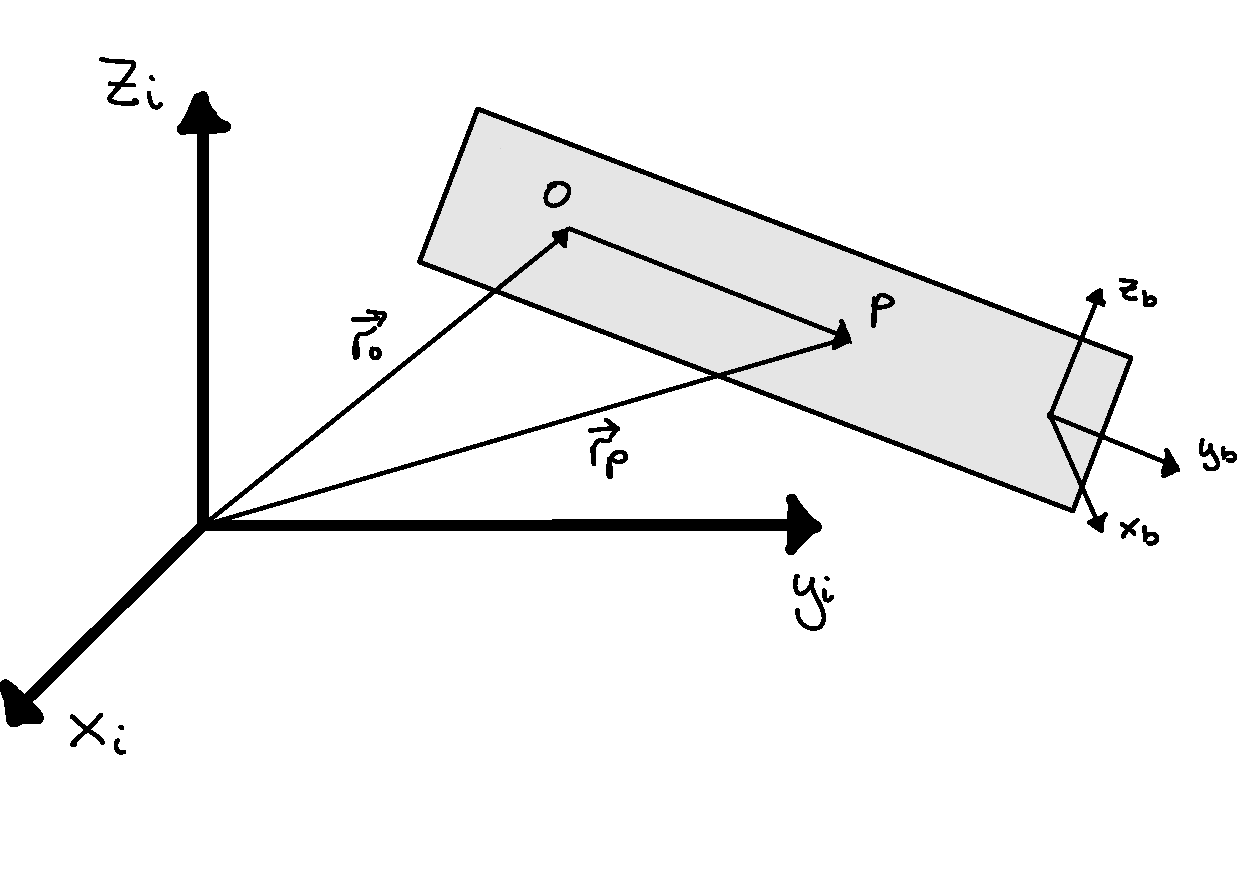
\includegraphics[width=\linewidth]{rigid-body.pdf}
    \label{fig:Test}
\end{Figure}

Velocity and Acceleration
\begin{align*}
    \vec{v}_p &:= \frac{{}^id}{dt}\vec{r}_p \\
              &= \vec{v}_o + \frac{{}^bd}{dt}\vec{r} + \vec{\omega}_{ib}\times\vec{r} \\
    \vec{a}_p &:= \frac{{}^id^2}{dt^2}\vec{r}_p \\
              &= \vec{a}_o + \frac{{}^bd^2}{dt^2}\vec{r} + 2\vec{\omega}_{ib}\times\frac{{}^bd}{dt}\vec{r} + \vec{\alpha}_{ib}\times\vec{r} + \vec{\omega}_{ib}\times(\vec{\omega}_{ib}\times\vec{r})
\end{align*}
The last three terms are, respectively, the coriolis acceleration, Transveral acceleration and Centripetal acceleration. Note that
\begin{align*}
    \vec{a}_o = \frac{{}^id}{dt}\vec{v}_o = \frac{{}^bd}{dt}\vec{v}_o + \vec{\omega}_{ib}\times\vec{v}_o
\end{align*}



\subsection{The center of mass} %% ------------------------- 6 . 13 ------------

The center of mass of a rigid body \(\mathcal{C}\) is defined to be
\begin{align*}
    \vec{r}_c := \frac{1}{m}\int_{\mathcal{C}}\vec{r}_p\,dm
\end{align*}
It can be shown that
\begin{align*}
    \vec{v}_c &= \frac{1}{m}\int_{\mathcal{C}}\vec{v_p}\,dm  &
    \vec{a}_c &= \frac{1}{m}\int_{\mathcal{C}}\vec{a_p}\,dm
\end{align*}
where \(c\) denotes \textit{center}



\setcounter{section}{7}
\setcounter{subsection}{1}
\subsection{Forces and torques} %% ------------------------- 7 . 2 -------------






\subsection{Newton-Euler Equations for rigid bodies} %% ---- 7 . 3 -------------



